\section{Log Extension} \label{sec:log}
Now we shift our focus on resilience to also include detection of misbehaving CT
logs.  The idea is an extension of our base design which relies on the
prerequisite that the CT landscape is modified to support SCT cross-logging.
Cross-logging refers to the idea of logging signed statements in other logs to
intertwine them, thus making it more difficult to get away with misbehavior.  We
use the general idea and apply it to SCTs.  This means that CTRs can disclose
SFOs to public scrutiny, forcing the CT logs in question to be accountable for
their SCTs.

\subsection{Design Sketch}
Figure~\ref{fig:ext-log} provides an overview of the extended design.  Tor
Browser submits presented SFOs probabilistically to CTRs that are selected
at random, and CTRs store the submitted SFOs before any auditing takes place.
Here, auditing refers to adding a complete SFO to an independent CT log.  While
phase~1 remains unchanged, there are minor changes to the Tor consensus,
phase~2, and phase~3.  The Tor consensus must include MMDs of CT logs that
Tor Browser recognizes, and CTRs should publish two additional metrics in the
extra-info document that are related to the threat of flooding.

\begin{figure*}
    \centering
    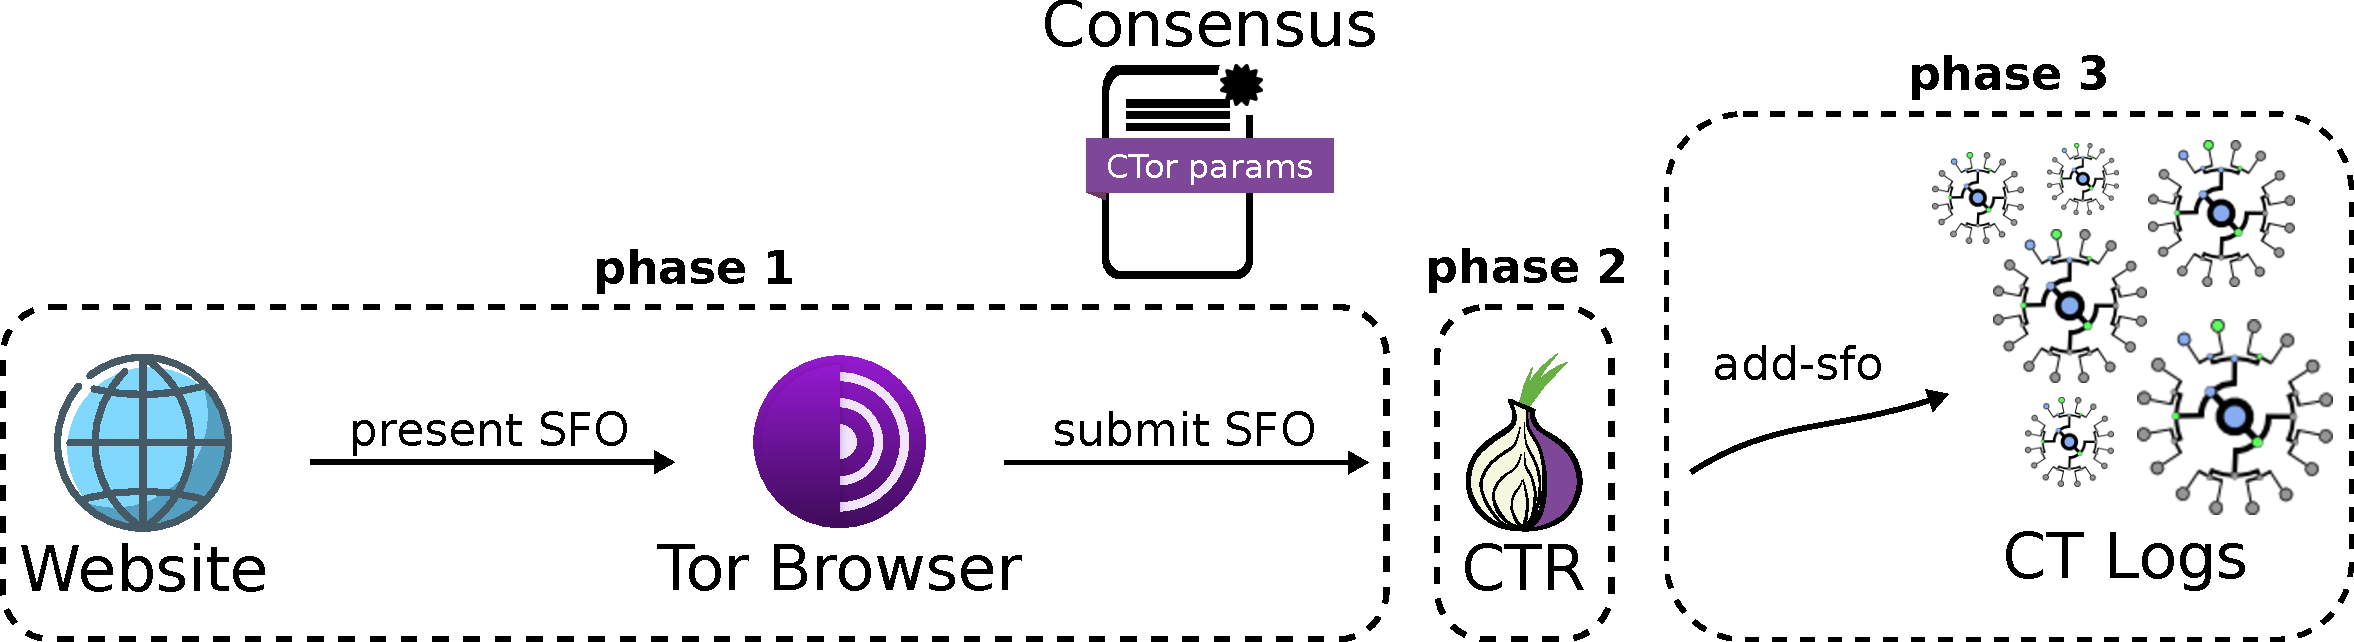
\includegraphics[width=0.85\textwidth]{img/design-log}
	\caption{The updated design of CTor to capture cryptographic evidence of CT
	log omission. The key difference to the previous design (shown in
	Figure~\ref{fig:design-ca}) is the new API call used at CT logs.}
    \label{fig:ext-log}
\end{figure*}

Starting backwards with phase~3, CT logs need an endpoint that accepts SCTs in
addition to certificate chains.  We refer to this endpoint as
\texttt{add-sfo}, and CTRs use it instead of \texttt{add-chain} or
\texttt{submit-entry}.  The added SCTs are of particular interest,
considering that they contain timestamps that reveal whether the issuing CT logs
violated their MMD promises by not incorporating a certificate chain on time.
Note that anyone can inspect the cross-logged SFOs, including existing CT
monitors, which in themselves prove whether a log misbehaved beyond doubt:
	an SCT is digitally signed by the issuing CT log, and
	it is cryptographically binding with regards to a certificate chain that
		is also publicly available.

To increase the probability of catastrophic impact for the attacker by detecting
omissions, it is paramount that there are no \emph{early signals} that
allow the CT logs in question to reactively merge certificate chains before
any MMD is violated.  Therefore, \texttt{audit\_after} timestamps should be
computed as in Figure~\ref{fig:audit-after} with regards to the SCT and MMD that
yields the largest value (phase~2).

%
% TODO:
% Think we need either 2*MMD as the log must produce an STH every MMD.  Or,
% have STHs in the consensus after all which would be more robust.
%

As discussed next, the possibility of larger \texttt{audit\_after} timestamps
introduces the threat of network-wide flushes.  To facilitate detection, CTRs
should publish received and deleted SFO-bytes in the extra-info document.  This
can be compared to existing extra-info metrics, such as a Tor relay's
\texttt{read-history}.

\subsection{Security Analysis}
% MISC notes
% - Network-wide flush, detectable but hard to attribute
% - Requires that the logs extend their APIs to accept SCT cross-logging
